\section{Contribution}
\label{sec:contribution}

In the scope of this thesis, we developed FESDData and FESDModel, or Fault estimation for Skeleton detection for data collection and model creation. FESDData is the tool that allows us to record, analyze and populate it with skeleton data using Nuitrack. FESDData is a tool that is designed to be easy to use and that can be used by anyone, and without much need for setup or tweaking.

FESDModel is the tool that allows us to train and evaluate the model. ... Still needs to be developed 

The code of this thesis is available on GitHub\footnote{\url{https://github.com/LeonardoPohl/FESD}}.

\subsection{Developed Software}

\textit{\textbf{UNSURE} Should I write about the software, explain the OpenGL implementation, the ImGui GUI and so on?}
\textit{\textbf{TODO} Change Screenshots to light mode to be consistent with the rest of the thesis (can wait until screenshots are final)}

\begin{figure}[ht]
  \centering
  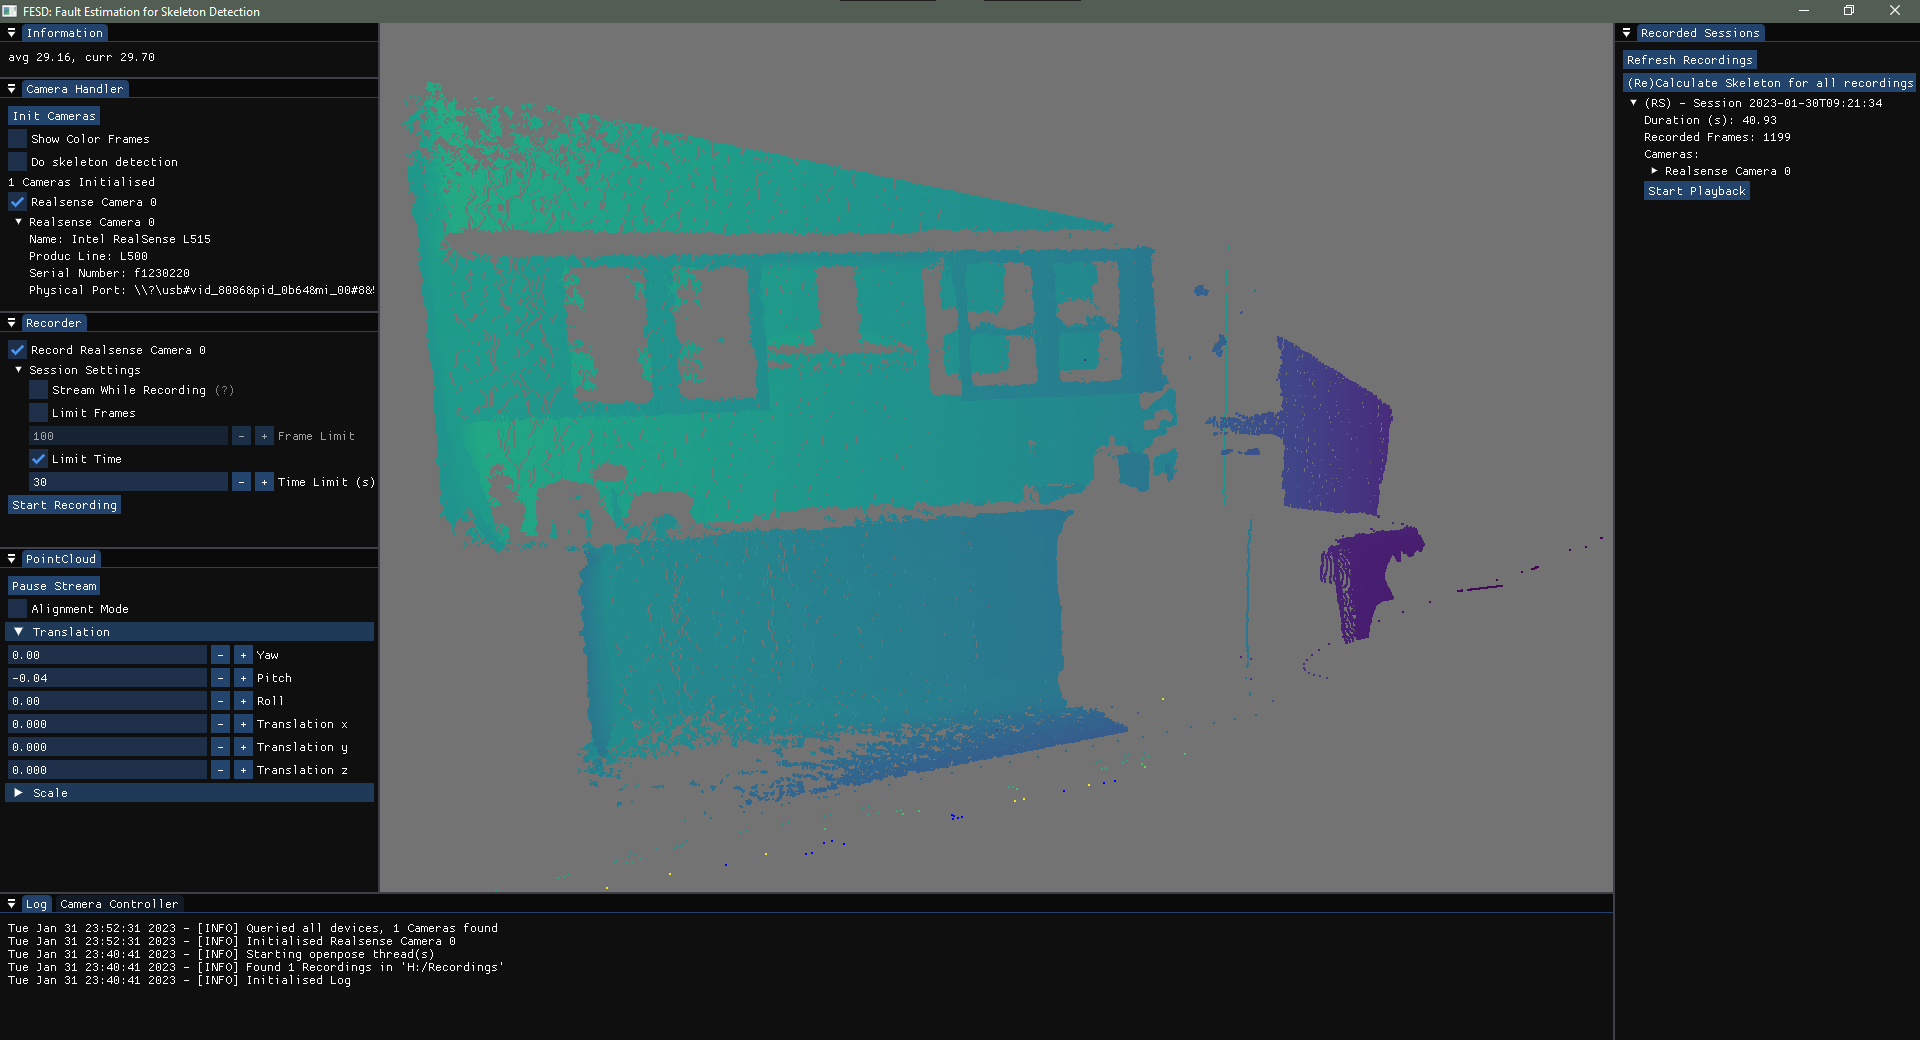
\includegraphics[width=\linewidth]{figures/FESD/all.png}
  \caption[FESD GUI]{A screenshot of the FESD GUI streaming a point cloud. The GUI is used to record and visualize the data, and to playback recordings to validate the data. The GUI is written in C++ using the ImGui framework. The Pointcloud is visualised using OpenGL and a glsl shader.}
  \label{fig:stream_gui}
\end{figure}

\subsection{Developed Model}

\subsection{Possible applications}

FESDModel and FESDData in combination offer users a way to collect and evaluate data for human pose estimation for very specific scenarios. For example in the case of SilverFit a number of exercises can be defined and recorded. The data can then be used to train a model that can be used to estimate the errors of the human pose that might arise with the specific exercise. This can then be used to improve the usage of the pose estimation model in the SilverFit application.